\documentclass{beamer}

\usetheme{Berlin}
\usecolortheme{Orchid}
\useoutertheme{miniframes}
\setbeamertemplate{navigation symbols}{}

\usepackage[utf8]{inputenc}
\usepackage[T1]{fontenc}
\usepackage{amsmath}
\usepackage{amssymb}
\usepackage{booktabs}
\usepackage{graphicx}
\graphicspath{{../images/}}

\usepackage{xcolor}
\usepackage{listings}
\usepackage{hyperref}
\usepackage{tikz}
\usetikzlibrary{arrows.meta,positioning,shapes.geometric,calc}

\lstset{
  language=Java,
  basicstyle=\ttfamily\small,
  keywordstyle=\color{blue},
  commentstyle=\color{gray},
  stringstyle=\color{teal},
  showstringspaces=false,
  columns=fullflexible,
  breaklines=true
}

% Per-slide source line (references shown on the slide itself).
\newcommand{\slidesources}[1]{%
  \vfill
  {\tiny\color{gray}\raggedright\sloppy\parbox{\linewidth}{Sources: #1}\par}%
}

% Unit-wise source strings for this subject (used by slides/notes).
% Path is relative to the lecture `latex/` folder (the compilation CWD).
% OOPS with Java (CSEG1044) — unit-wise sources
%
% These are short, student-facing reference strings intended to be used with:
%   - \slidesources{...}  (in beamer slides)
%   - \notesources{...}   (in lecture notes)
%
% Style inspiration: other subjects in My-Subjects/ use semicolon-separated sources
% and include an "accessed" date for web documentation.

\newcommand{\OOPSUnitISources}{Schildt, \textit{Java: A Beginner's Guide} (10e), McGraw-Hill (Java fundamentals + OOP basics).; Oracle Java Tutorials: Getting Started + Language Basics + Classes and Objects (accessed \today).; Java SE API docs (e.g., \texttt{String}, \texttt{Scanner}) (accessed \today).}

\newcommand{\OOPSUnitIISources}{Schildt, \textit{Java: The Complete Reference} (12e), McGraw-Hill (classes, inheritance, packages, interfaces).; Bloch, \textit{Effective Java} (3e), Addison-Wesley, 2018 (design choices; interfaces vs abstract classes).; Oracle Java Tutorials: Classes and Objects + Interfaces + Packages (accessed \today).; Java SE API docs (e.g., \texttt{Comparable}, \texttt{Runnable}) (accessed \today).}

\newcommand{\OOPSUnitIIISources}{Schildt, \textit{Java: The Complete Reference} (12e) (nested/inner classes, exceptions, threads, I/O).; Oracle Java Tutorials: Nested Classes + Exceptions + Concurrency + Basic I/O (accessed \today).; Java SE API docs (e.g., \texttt{Thread}, \texttt{AutoCloseable}) (accessed \today).}

\newcommand{\OOPSUnitIVSources}{Schildt, \textit{Java: The Complete Reference} (12e) (generics, lambdas, Swing, JDBC).; Bloch, \textit{Effective Java} (3e) (generics + lambdas).; Oracle Java Tutorials: Generics + Lambda Expressions + Swing + JDBC Basics (accessed \today).; Java SE API docs (e.g., \texttt{java.util.function}, \texttt{javax.swing}, \texttt{java.sql}) (accessed \today).}

\newcommand{\OOPSUnitVSources}{Schildt, \textit{Java: The Complete Reference} (12e) (Collections Framework + wrapper classes).; Oracle Java docs: Collections Framework overview (accessed \today).; Java SE API docs (\texttt{java.util} collections; wrapper classes in \texttt{java.lang}) (accessed \today).}

\newcommand{\OOPSUnitVISources}{Git SCM: \textit{Pro Git} (2e) (version control workflow), accessed \today.; GitHub Docs (repositories, issues, pull requests), accessed \today.; Oracle Java Tutorials: Swing + JDBC (accessed \today).; JUnit 5 User Guide (accessed \today).; Apache Maven Project: Getting Started (accessed \today).; Gradle User Manual: Getting Started (accessed \today).; UML class diagrams: UML 2.x overview/spec (accessed \today).}

\newcommand{\OOPSMiscWhyInterfacesSources}{Schildt, \textit{Java: The Complete Reference} (12e) (interfaces).; Bloch, \textit{Effective Java} (3e) (prefer interfaces where appropriate).; Oracle Java Tutorials: Interfaces (accessed \today).; Java SE API docs (e.g., \texttt{Comparable}, \texttt{Runnable}) (accessed \today).}



\title[OOPS with Java]{Object Oriented Programming (CSEG1044)}
\subtitle{Unit 06 -- Lecture 05: Swing UI Panels + Integration}
\author{Tofik Ali}
\institute{School of Computer Science, UPES Dehradun}
\date{\today}

\begin{document}

\begin{frame}[fragile]
  \titlepage
  \vspace{0.5em}
  \slidesources{\OOPSUnitVISources}
\end{frame}

\begin{frame}{Quick Links}
  \centering
  \hyperlink{sec:overview}{\beamerbutton{Overview}}\hspace{0.6em}
  \hyperlink{sec:concepts}{\beamerbutton{Key Topics}}\hspace{0.6em}
  \hyperlink{sec:demo}{\beamerbutton{Demo}}\hspace{0.6em}
  \hyperlink{sec:summary}{\beamerbutton{Summary}}
  \slidesources{\OOPSUnitVISources}
\end{frame}

\begin{frame}{Agenda}
  \tableofcontents
  \slidesources{\OOPSUnitVISources}
\end{frame}

\section{Overview}
\label{sec:overview}

\begin{frame}{Learning Outcomes}
  \begin{itemize}[<+->]
    \item Plan screens/panels and choose layout managers.
    \item Implement events that call service/DAO cleanly.
    \item Complete Deliverable-4: one end-to-end UI flow connected to persistence.
  \end{itemize}
  \slidesources{\OOPSUnitVISources}
\end{frame}

\begin{frame}{Where we are in the capstone}
  \begin{itemize}[<+->]
    \item Deliverable-0: team + repo + backlog
    \item Deliverable-1: requirements + use cases
    \item Deliverable-2: class design + packages
    \item Deliverable-3: DB schema + DAO CRUD
    \item \textbf{Now: Deliverable-4} UI $\rightarrow$ DB $\rightarrow$ UI refresh
  \end{itemize}
  \slidesources{\OOPSUnitVISources}
\end{frame}

\begin{frame}{Deliverable-4 (today)}
  \begin{itemize}[<+->]
    \item At least 2 screens/panels (list + form).
    \item One complete flow: Add (or Book) $\rightarrow$ save in DB $\rightarrow$ refresh list.
    \item Validations + user-friendly messages.
    \item Evidence: issues + PR + short README ``how to run''.
  \end{itemize}
  \slidesources{\OOPSUnitVISources}
\end{frame}

\section{Key Topics}
\label{sec:concepts}

\begin{frame}{Unit 06: Capstone Project}
  \begin{itemize}[<+->]
    \item Lecture focus: Swing UI Panels + Integration
  \end{itemize}
  \slidesources{\OOPSUnitVISources}
\end{frame}

\begin{frame}{Today: Roadmap}
  \begin{itemize}[<+->]
    \item Screen plan + navigation (what panels do we need?)
    \item Layout managers + event handling pattern
    \item Clean integration: UI vs service vs DAO; validation + messages
  \end{itemize}
  \slidesources{\OOPSUnitVISources}
\end{frame}

\begin{frame}{Screen plan example (Resource Booking)}
  \begin{itemize}[<+->]
    \item Resource list (table) + ``Add Resource'' (dialog/form)
    \item Booking form (select resource, time, user)
    \item Booking list (table)
  \end{itemize}
  \vspace{0.6em}
  \textbf{Navigation choices:}
  \begin{itemize}[<+->]
    \item \texttt{CardLayout} to switch screens
    \item \texttt{JTabbedPane} for independent pages
  \end{itemize}
  \slidesources{\OOPSUnitVISources}
\end{frame}

\begin{frame}{Layout managers (cheat sheet)}
  \begin{itemize}[<+->]
    \item \texttt{BorderLayout}: main structure (North/West/Center)
    \item \texttt{BoxLayout}: vertical stacks
    \item \texttt{GridLayout}: uniform grids
    \item \texttt{GridBagLayout}: aligned forms (labels + fields)
    \item \texttt{CardLayout}: multi-screen apps
  \end{itemize}
  \textbf{Rule:} avoid \texttt{null} layout.
  \slidesources{\OOPSUnitVISources}
\end{frame}

\begin{frame}[fragile]{Event handler pattern (keep it short)}
\begin{lstlisting}
btnSave.addActionListener(e -> {
    try {
        service.createResource(
            txtName.getText(),
            txtType.getText(),
            Integer.parseInt(txtCap.getText())
        );
        JOptionPane.showMessageDialog(this, "Saved!");
        refreshTable();
    } catch (Exception ex) {
        showError(ex);
    }
});
\end{lstlisting}
  \begin{itemize}[<+->]
    \item UI reads inputs, service validates, DAO persists.
    \item UI shows message and refreshes view.
  \end{itemize}
  \slidesources{\OOPSUnitVISources}
\end{frame}

\begin{frame}{Layering (what goes where?)}
  \centering
  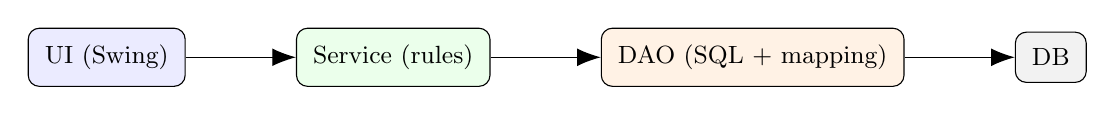
\begin{tikzpicture}[node distance=1.4cm, every node/.style={font=\small}]
    \node[draw, rounded corners, fill=blue!8, inner sep=6pt] (ui) {UI (Swing)};
    \node[draw, rounded corners, fill=green!8, right=of ui, inner sep=6pt] (svc) {Service (rules)};
    \node[draw, rounded corners, fill=orange!10, right=of svc, inner sep=6pt] (dao) {DAO (SQL + mapping)};
    \node[draw, rounded corners, fill=gray!10, right=of dao, inner sep=6pt] (db) {DB};
    \draw[-{Latex[length=3mm]}] (ui) -- (svc);
    \draw[-{Latex[length=3mm]}] (svc) -- (dao);
    \draw[-{Latex[length=3mm]}] (dao) -- (db);
  \end{tikzpicture}

  \vspace{0.6em}
  \begin{itemize}[<+->]
    \item UI: \textit{no SQL}; convert fields + show results.
    \item Service: validations; business rules (e.g., no overlap).
    \item DAO: JDBC code only.
  \end{itemize}
  \slidesources{\OOPSUnitVISources}
\end{frame}

\begin{frame}{Validation + user messages}
  \begin{itemize}[<+->]
    \item UI validation: required fields + parsing (numbers/dates).
    \item Service validation: full rules (start before end; capacity $>$ 0).
    \item Use \texttt{JOptionPane} for readable messages.
  \end{itemize}
  \textbf{Tip:} never show stack traces to users.
  \slidesources{\OOPSUnitVISources}
\end{frame}

\begin{frame}{EDT rule (avoid frozen UI)}
  \begin{itemize}[<+->]
    \item Swing is single-threaded (EDT paints + handles clicks).
    \item Slow DB calls on EDT freeze the UI.
    \item If needed: use \texttt{SwingWorker} for background DB calls.
  \end{itemize}
  \slidesources{\OOPSUnitVISources}
\end{frame}

\section{Demo / Example}
\label{sec:demo}

\begin{frame}{Demo plan (10--15 mins)}
  \begin{enumerate}[<+->]
    \item Create \texttt{ResourceListPanel} with a \texttt{JTable}.
    \item Add an ``Add Resource'' dialog (or panel).
    \item On save: call service $\rightarrow$ DAO insert.
    \item Refresh table from DB.
  \end{enumerate}
  \slidesources{\OOPSUnitVISources}
\end{frame}

\begin{frame}{Mini Exercises (5 mins)}
  \begin{enumerate}[<+->]
    \item Which layer should enforce ``booking end after start''?
    \item If \texttt{Integer.parseInt} fails, where do you handle it?
    \item What is the EDT and why does it matter?
  \end{enumerate}
  \slidesources{\OOPSUnitVISources}
\end{frame}


\section{Summary}
\label{sec:summary}

\begin{frame}{Key Takeaways}
  \begin{itemize}[<+->]
    \item Plan screens first; use layout managers for scalable UI.
    \item Keep button handlers short; call service methods.
    \item Deliverable-4 proves your app works end-to-end.
  \end{itemize}
  \slidesources{\OOPSUnitVISources}
\end{frame}

\begin{frame}{Checkpoint Questions}
  \begin{enumerate}[<+->]
    \item Why should Swing UI avoid SQL code?
    \item What is a good use of \texttt{CardLayout}?
    \item How do you refresh a table after inserting into DB?
  \end{enumerate}
  \slidesources{\OOPSUnitVISources}
\end{frame}

\begin{frame}{Next Lecture Preview}
  \textbf{Next:} Testing + build/artifacts + final demo (Deliverable-5)
  \vspace{0.6em}
  \begin{itemize}[<+->]
    \item Add JUnit tests for service rules.
    \item Package a runnable artifact and prepare a demo script.
  \end{itemize}
  \slidesources{\OOPSUnitVISources}
\end{frame}

\end{document}
